\chapter{Einführung}
\label{chap:einfuehrung}

\section{Allgemeines zu dieser Vorlage}
\label{sec:Vorlage}
Dieses \LaTeX-Template soll die Erstellung von Abschlussberichten erleichtern. Es wurde versucht, in diesem Dokument die wichtigsten Elemente eines Abschlussberichtes beispielhaft zu verwenden.
Dazu geh"oren Listen, Tabellen, Bilder, w"ortliche und nicht-w"ortliche Zitate, Zitierweisen von Zeitschriftenartikeln, B"uchern, Abschluss("s)arbeiten und Webseiten, Gleichungen und Referenzierungen von Kapiteln und Grafiken.

\paragraph{Vollst"andigkeit}
Die Verwendung der Elemente erhebt keinen Anspruch auf Vollst"andigkeit.
Allerdings bietet das Internet\cite{onlineLatexHilfe} viele Hilfestellungen f"ur \LaTeX, weshalb es kein Problem ist falls nicht bekannt ist, wie $\gamma$ im Mathematik-Modus geschrieben wird.

\section{Meine Arbeit ist zu kurz. Was tun?}
\label{sec:ZuKurz}

Sollten es Schwierigkeiten geben die vorgeschriebene L"ange zu erreichen, vergr"o"sern Sie nicht die Graphiken unangemessen oder schinden ansonsten Seiten, sondern denken "uber folgende Fragen nach:
\begin{enumerate}
\item Habe ich die Literatur zu meinem Thema ausreichend gew"urdigt?
\item Habe ich eine Hinleitung zum Kernthema so geschrieben, dass meine Studienkolleginnen und -kollegen -- ohne Wikipedia zu bem"uhen -- folgen k"onnen?
\item Habe ich die Kernpunkte detailliert genug geschildert?
\item Habe ich alle sinnvollen Experimente tats"achlich durchgef"uhrt, eine Hypothese daran verifiziert oder falsifiziert, das jeweilige Ergebnis nachvollziehbar beschrieben und diskutiert?
\item Habe ich "uber den Tellerrand hinausgesehen und in einem ausf"uhrlichen Ausblick k"unftige sinnvolle Schritte thematisiert?
\end{enumerate}



\chapter{Beispiele}
\label{chap:Beispiele}
Im zweiten Kapitel werden einige Beispiele gezeigt, die f"ur die Arbeit relevant sein können.

\section{Referenzen innerhalb des Dokuments}
Jedes Strukturelement, wie z.B.
\begin{itemize}
\item section
\item subsection
\item chapter
\item usw \dots
\end{itemize}
sollte mit einem \textit{Label} versehen werden. Damit kann an beliebiger Stelle in der Arbeit auf den Abschnitt verwiesen werden.

\FloatBarrier
\begin{figure}[htb]
\begin{lstlisting}[backgroundcolor={\color{white}},
basicstyle={\normalsize\sffamily}]	

	\label{chap:myFirstChapter}
            
\end{lstlisting}
  \caption[Referenzieren auf ein Kapitel (chapter)]{Mit diesem Code wird auf das zuvor vergebene Label eines Kapitels (chapter) verwiesen.}
\label{lst:literaturenquelle}
\end{figure}



\section{Einbinden externer Dateien}
Es besteht die Möglichkeit, einzelne LaTex-Dateien manuell einzubinden. Dies hat den Vorteil, dass die Kapitel logisch und physisch voneinander getrennt werden können, was bei der Arbeit mit einem Repository mit mehreren Teilnehmern von Vorteil ist.\\

Jede einzelne \textit{.tex}-Datei muss hierzu in der \textit{Masterdatei} referenziert werden. In Abbildung \ref{lst:extDateieinbinden} wird die Datei namens \textit{01\_titel.tex} eingebunden.

\FloatBarrier
\begin{figure}[htb]
\begin{lstlisting}
;
;	% Titelblatt-Datei einbinden. 
;	% Hier muessen der Dateiname und der Pfad stimmen!
;	\include{01_titel}
;           
\end{lstlisting}
  \caption[Einbinden einer externen Datei]{Einbinden einer externen Datei. Der Dateiname muss hier exakt, jedoch ohne Dateiendung angegeben werden.}
\label{lst:extDateieinbinden}
\end{figure}


\section{Einbinden von Grafiken}
\label{sec:EinbindenVonGrafiken}

% ### EINBINDEN EINER GRAFIK ###
\FloatBarrier
\begin{figure}[htb]
  \centering  
  
\includegraphics[scale=0.3]{img/kein_bild_vorhanden.eps}
  \caption[Beispiel für das Einbinden einer Grafik.]{Lange Beschreibung für das Einbinden einer Grafik. Die Kurzbeschreibung für das Abbildungsverzeichnis befindet sich davor in eckigen Klammern.} 
  \label{fig:kein_bild_vorhanden}
\end{figure}

An dieser Stelle befindet sich ein Beispiel, wie ein interner Verweis aufgebaut ist (siehe Abbildung \ref{fig:kein_bild_vorhanden}), der die Grafik verlinkt \dots

\section{Einbinden von PDF-Dateien}
\label{sec:PDFeinfuegen}
Das Keyword \textit{trim} schneidet den gewünschten Ausschnitt der Datei passend zu. Dabei ist die Reihenfolge der Seiten zu beachten. Zuerst wird links, dann unten, dann rechts und zuletzt die obere Seite angepasst. Zum Schluss muss das Argument \textit{clip} angefügt werden, ansonsten hat der Trick keinen Effekt.

% ### EINBINDEN VON PDFs
\begin{figure}[htb]
  \centering  
  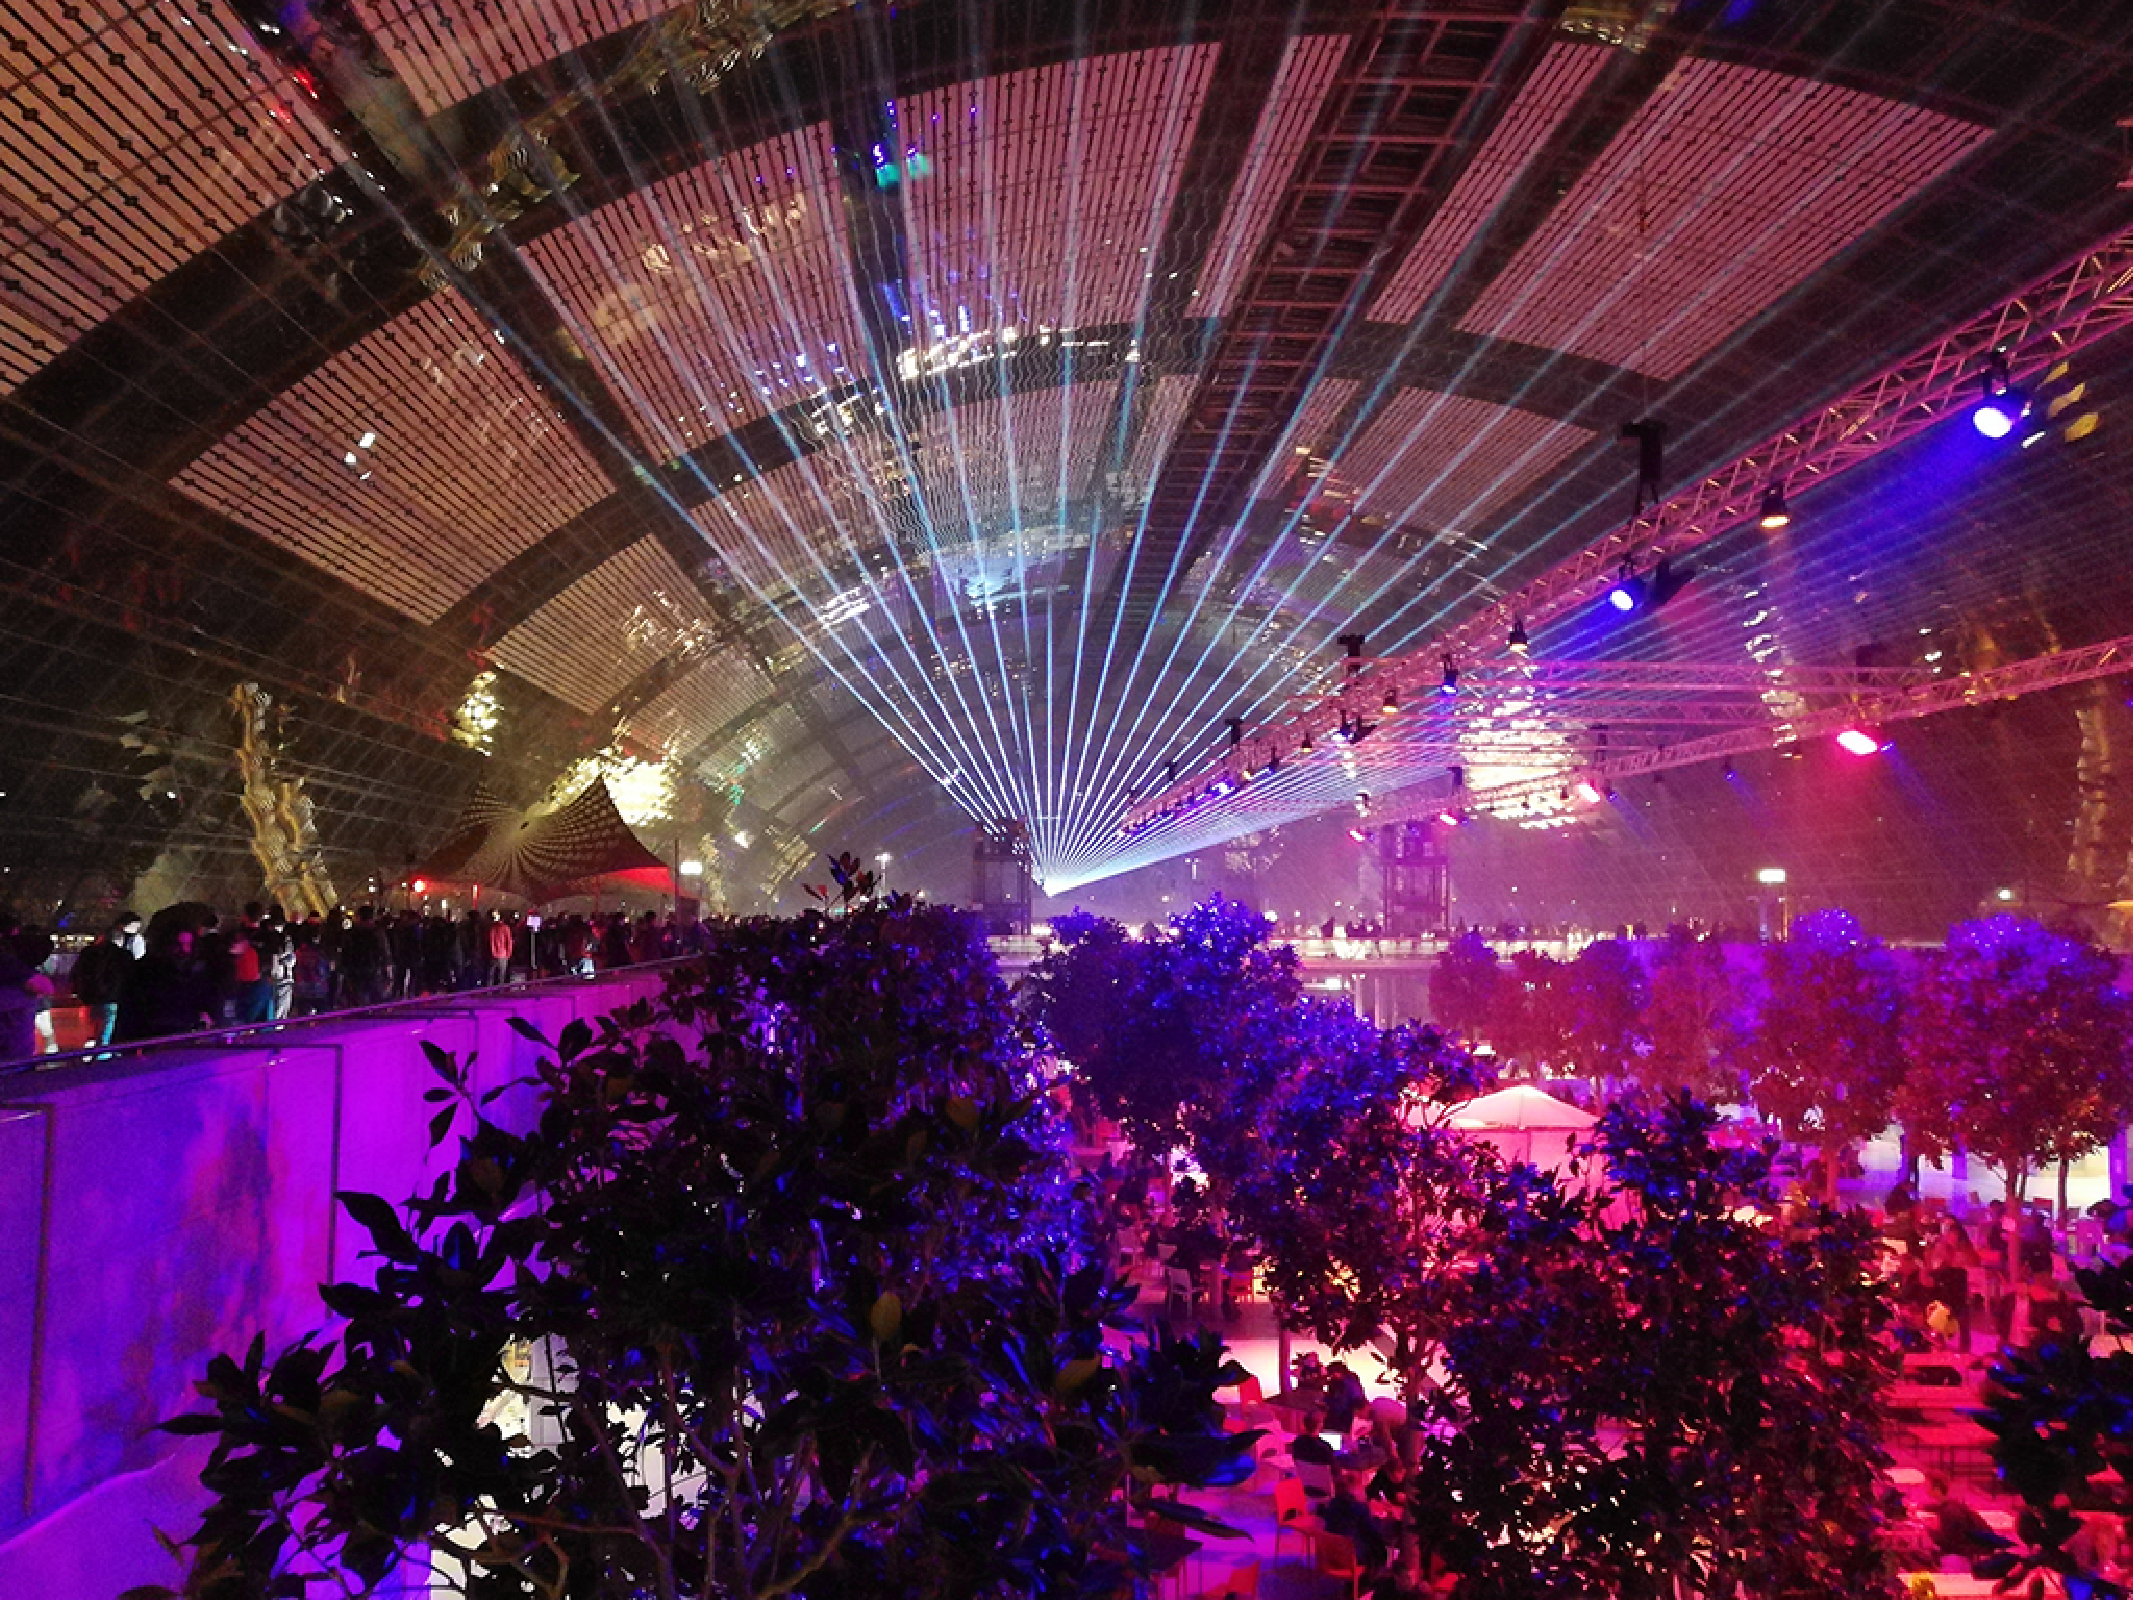
\includegraphics[width=0.8\textwidth, trim = 10mm 10mm 10mm 10mm, clip]{img/34c3.pdf}
  \caption[Beispiel für das Einbinden einer PDF-Datei.]{Das Bild wurde zentriert, 10mm auf jeder Seite zugeschnitten und mit einer Breite von 80 \% der Textbreite skaliert.} 
  \label{fig:34c3}
\end{figure}
\FloatBarrier



\section{Tabellen}
\label{sec:Tabellen}
Tabellen sind mit etwas Aufwand zu verwalten. Der grobe Aufbau sollte vor Beginn klar sein. Spalten im Nachhinein zu vertauschen, bedeutet einen vergleichsweise großen Aufwand.

\subsection{Tabelle 1 - einfach}
\label{subsection:Tabelle1}

In Tabelle \ref{tab:Tabelle1} ist eine einfache Tabelle zu sehen.\\

\newcolumntype{b}{X}
\newcolumntype{s}{>{\hsize=.2\hsize}X}
\begin{table}[H]
\begin{tabularx}{\textwidth}{sb}
%{X|X}
\textbf{Spalte1} & \textbf{Spalte2}\\
\hline

Zelle11 & Zelle12.  \\ \hline

Zelle21 & Zelle22. \\ \hline

\end{tabularx}
\caption[Einfache Tabelle]{Das ist eine einfache Tabelle, die zwei Spalten und drei Zeilen besitzt.
\label{tab:Tabelle1}}
\end{table}
\FloatBarrier

\subsection{Tabelle 2 - komplex}
\label{subsection:Tabelle2}

In Tabelle \ref{tab:Tabelle2} ist eine komplexere Tabelle zu sehen.\\

\begin{table}[H]\vspace{1ex}\centering
\begin{tabular*}{12cm}{ll|@{\extracolsep\fill}cccc}
&&\multicolumn{4}{c}{Verfahren} \\
&& A  & B &  C & D\\\hline
\multirow{5}*{\rotatebox{90}{Datens"atze}}
& Proband 1 &  negativ  & negativ & negativ & negativ  \\%\cline{2-6}
& Proband 2 &  negativ  & negativ & negativ & negativ  \\%\cline{2-6}
& Proband 3 &  negativ  & negativ & negativ & negativ  \\%\cline{2-6}
& Proband 4 &  negativ  & negativ & \textbf{positiv} & bla \\%\cline{2-6}
& Proband 5 &  negativ  & negativ & negativ & negativ  \\\hline
\end{tabular*}
\caption[Komplexe Tabelle]{Das ist ein Beispiel f"ur eine recht komplexe Tabelle.
Nicht der gesamte Text der Tabellenunterschrift sollte im Tabellenverzeichnis auftauchen.
Hier wurde der beste Wert \textbf{fett} markiert.
\label{tab:Tabelle2}}
\vspace{2ex}\end{table}

\subsection{Tabelle 3 - mit Minipage}
\label{subsection:Tabelle3}
Referenzen auf Fußnoten \textit{innerhalb} einer Tabelle werden erst vollständig angezeigt, wenn die Tabelle von einer \textbf{Minipage} eingefasst ist. Die Fußnoten folgen jedoch dann direkt hinter der Tabelle.

\FloatBarrier
\newcolumntype{a}{>{\hsize=.8\hsize}X}
\newcolumntype{g}{>{\hsize=.5\hsize}X}
\newcolumntype{o}{>{\hsize=.1\hsize}X}
\begin{table}[H]
\begin{minipage}{\textwidth}
\begin{tabularx}{\textwidth}{ago}
%{X|X}
\textbf{Spalte1} &  \textbf{Spalte2} & \textbf{Spalte3}\\
\hline

Lorem ipsum dolor sit amet, consetetur sadipscing elitr. & Vendor\footnote{\url{https://www.amazon.de}, Aufruf am 04.03.2018} & 33,99  \\ \hline

Lorem ipsum dolor sit amet, consetetur sadipscing elitr. & Vendor\footnote{\url{https://www.amazon.de}, Aufruf am 04.03.2018} & 33,47 \\ \hline

Lorem ipsum dolor sit amet, consetetur sadipscing elitr. & Vendor\footnote{\url{https://www.amazon.de}, Aufruf am 04.03.2018} & 42,99 \\ \hline 

\end{tabularx}
\caption[Minipage in einer Tabelle]{Das ist ein Beispiel f"ur eine Tabelle, die von einer Minpage eingefasst wird, um alle Referenzen der Fußzeile anzuzeigen.}
\label{tab:Tabelle3}
\end{minipage}
\end{table}
\FloatBarrier


\subsection{Tabelle 4 - mit Parbox}
\label{subsection:Tabelle4}
Zu breite Wörter oder Sätze innerhalb einer Zelle einer Tabelle können mit einer sogenannten \textbf{Parbox} zu einem Zeilenumbruch gezwungen werden, wie in Tabelle \ref{tab:Tabelle4} zu sehen. Auch die Zellen- bzw. Spaltenbreite kann durch die Parbox bestimmt werden, ist dann jedoch nicht mehr relativ.

\begin{table}[H]\centering
\begin{tabularx}{\textwidth}{l l l} 			
\parbox[t]{2.5cm}{\textbf{Spalte1}}	& \parbox[t]{9cm}{\textbf{Spalte2}}                                 			& \textbf{Spalte3}	\\\hline

\parbox[t]{2.5cm}{Zelle1}             		& \parbox[t]{9cm}{Zelle2}                                                 	&   Zelle3                 	\\ 

\parbox[t]{2.5cm}{Zelle1}    	   	    	& \parbox[t]{9cm}{Lorem ipsum dolor sit amet, consetetur sadipscing elitr, sed diam nonumy eirmod tempor invidunt ut labore et dolore magna aliquyam erat, sed diam voluptua. At vero eos et accusam et justo duo dolores et ea rebum. )}	& Zelle3        \\

\parbox[t]{2.5cm}{Zelle1}             		& \parbox[t]{9cm}{Zelle2}                                                 	&   Zelle3                 	\\ 

\end{tabularx}
\caption[ParBox in einer Tabelle]{Die Breite eines Zelleninhalts kann mit einer Parbox begrenzt werden.}
\label{tab:Tabelle4}
\end{table}



\section{Aufz"ahlungen}
\label{sec:Aufzaehlungen}

\subsection{Punkt}
\label{subsec:Punkt}

% ### VERSCHACHTELTE AUFZAEHLUNGEN ###
\begin{itemize}
\item Stichpunkt 1
\item Stichpunkt 2
\begin{itemize}
\item Unterpunkt 1
\item Unterpunkt 2
\end{itemize}
\end{itemize}

\subsection{Zahlen}
\label{subsec:Zahlen}

\begin{enumerate}
\item Nummerierter Stichpunkt 1
\item Nummerierter Stichpunkt 2
\end{enumerate}


\section{Mathematische Formeln}
\section{sec:MatheFormeln}
Solange die Formeln in der Ausarbeitung hergeleitet werden muss eine Quelle angegeben werden. Im folgenden wird ein Beispiel einer Angabe von einer Formel vorgestellt \ref{Formel:Binomailfilter5x5}:


\begin{figure}[htbp]
  \centering 
   \[
   h_{ga 5}(x,y) = \frac{1}{256} \begin{bmatrix}
	1 & 4  & 6 & 4 & 1 \\
	4 & 16 & 24 & 16 & 4 \\
	6 & 24 & 36 & 24 & 6 \\
	4 & 16 & 24 & 16 & 4 \\
	1 & 4  & 6 & 4 & 1
	\end{bmatrix} 
   \]
   \renewcommand\figurename{Formel}
   \caption[Formel für einen 5x5 Binomialfilter]%
  {In der Abbildung ist ein Gaußfilter mit dem Kernelgröße 5x5 zu sehen \cite{Segmentierung:DigitaleBildvearbeitung}.}    
  \label{Formel:Binomailfilter5x5}        
\end{figure}



\section{Fu{\ss}zeile}
\label{sec:Fusszeile}

Eine Quelle in der Fußzeile lässt sich \textit{folgendermaßen}\footnote{\url{http://my/url.com}, (Zugriff am 17.10.2017)} realisieren. Das Thema \textbf{Zitierungen} wird später im Dokument behandelt.

\section{Listings}
\label{sec:Listings}

\paragraph{Quellcode in Listings}
Quellcode kann durchaus \textbf{sparsam dosiert} in der Arbeit auftauchen.
Das jedoch nicht vollst"andig und als Anhang (siehe Anhang \ref{cap:Anhang}), sondern in sinnvollen Ausschnitten, wenn anhand des Code-Fragments ein Sachverhalt erl"autert werden soll.

\subsection{Listing 1}
\label{subsec:Listing1}

\FloatBarrier
\begin{figure}[htb]
\begin{lstlisting}[language=C++, breaklines=true, basicstyle=\small, numbers=none]
// Das ist ein Beispiel fuer ein Codefragment
int a = 7;
int b = 3;
int c = 10;
a *= 2;
c -= b + a++;
std::cout << "c = " << c << std::endl;
\end{lstlisting}
  \caption[Beispiel eines einfachen Codefragments.]{Ein einfaches Codefragment, das eine mathematische Berechnung demonstriert.}
\label{lst:Codefragment}
\end{figure}


\subsection{Listing 2}
\label{subsec:Listing 2}

Das Listing \ref{lst:Diagramm} ist eines, das ASCII-Code einbettet.

% ### Das hier ist ein Listing, das ASCII-Code einbettet ###
\FloatBarrier
\begin{figure}[htb]
\begin{lstlisting}[backgroundcolor={\color{white}},
basicstyle={\normalsize\sffamily},
breaklines=true,
frame={bottomline,topline, rightline},
language=HTML,
numbers=left,
showstringspaces=false,
xleftmargin=22pt]	
; This is the description of a test case.
;
;           .------------------------------.
;           |          Start [0]           |
;           '------------------------------'
;                           |
;                           v
;       .---------------------------------------.
;       |             Some content		        |
;       '---------------------------------------'
;                           |
;                           v
;           .------------------------------.
;           |          Return [1]          |
;           '------------------------------'
\end{lstlisting}
  \caption[Ein Listing mit ASCII-Code und Zeilennummern]{Dieses Listing kann verwendet werden, um ein einfaches Diagramm zu erstellen oder Code einzubinden. Die Formatierungsparameter sind zahlreich verfügbar.}
\label{lst:Diagramm}
\end{figure}




\section{Listing an gewünschter Stelle einfügen}
\label{sec:FigurHierEinfuegen}
Um ein Listing an einer bestimmten Stelle einzubinden, muss man den Parameter [H] verwenden.

\FloatBarrier
\begin{figure}[htb]
\begin{lstlisting}[backgroundcolor={\color{white}},
basicstyle={\normalsize\sffamily},
breaklines=true,
frame={bottomline,topline, rightline},
language=HTML,
numbers=left,
showstringspaces=false,
xleftmargin=22pt]	
; 
;	\begin{figure}[htb]
;	...
;	\end{figure}
;
\end{lstlisting}
  \caption{Beschreibung des Listings.}
\label{lst:FigurGenauHier}
\end{figure}

\section{Unterstreichen und durchstreichen von Texten}
\label{sec:Durchstreichen}

Es stehen folgende Befehle zur Verfügung:\\

\begin{itemize}
\item \uline{important}  % unterstreichen
\item \uuline{urgent}    % doppelt unterstreichen
\item \uwave{boat}       % unterschlängeln
\item \sout{wrong}       % durchstreichen
\item \xout{removed}     % ausstreichen mit //////.
\end{itemize}


\section{Formeln}
\label{sec:Formeln}

Formeln werden nach folgendem Schema angegeben:

\begin{equation}
g = n\cdot l_n + l_i + l_l + 1.
\label{gle:Laenge}
\end{equation}




\section{Zitierung}\label{zitierung}

Es ist verpflichtend, alle Quellen und Hilfmittel anzugeben, die verwendet werden.
Dabei ist die w"ortliche Zitierung in der Informatik selten, schon deshalb, weil viele Quellen englischsprachig sind und ein englisches w"ortliches Zitat in einer deutschen Arbeit keinen Sinn macht.
Meist werden Gedanken, Ideen und Methoden aus Quellen entnommen.
Das Zitat kommt dann an den Schlus des letzten Satzes des Abschnittes, der z.B. die Methode beschreibt \cite{wissentschaftlichesArbeitMitLatex}.
Bitte beachten Sie, dass das Zitat \textbf{vor} dem abschli"senden Punkt erscheint und nicht danach!

Alternativ wird zu Beginn oder am Ende der Beschreibung der Methode die Quelle mit Hilfe einer Phrase wie:
\begin{quote}
Angreifer, die Zugang zum PC haben m"ochten nutzen die Anwendungen von dem Benutzer, die selten bis garnicht verwendet werden. Sobald der Benutzer diese Hintert"uren geschlossen hat kann man sich mit den seinen eigenen Daten sicherer f"uhlen \cite{ctWindowsEinfachAbsichern}.
\end{quote}


Als ein hilfreiches Werkzeug zum Auffinden von wissenschaftlichen Artikeln hat sich \url{http:\\\\scholar.google.com} erwiesen.

\paragraph{Zitierung von Internetseiten}
Grunds"atzlich ist das Zitieren von Internetseiten so weit wie m"oglich zu vermeiden.
Internetseiten k"onnen pl"otzlich offline sein, der Inhalt kann sich "andern, manchmal ist der Autor unklar.
Genau das Gegenteil erwartet man von einer \emph{zitierf"ahigen} Quelle.
Dennoch l"a"st sich der Hinweis auf eine Internetseite manchmal nicht vermeiden.
In diesen F"allen versuchen Sie, den Autor herauszufinden und in die Quellenangabe einzuf"ugen.
Wichtig ist der Hinweis auf das letzte Zugriffdatum \cite{zitieren13}.
Au"serdem wird meistens erwartet die Seiten lokal zu speichern und ebenso in elektronischer Form zu der Arbeit hinzuzuf"ugen.

Besonders Wikipedia-Seiten sind kritisch zu bewerten. In Wikipedia selbst ist zu lesen:
\begin{quote}
\glqq In wissenschaftlichen Arbeiten sollte auf das Zitieren von Wikipedia-Artikeln nach M"oglichkeit verzichtet werden, da keine Garantie f"ur den Inhalt gegeben werden kann.
Zudem folgt Wikipedia derzeit nur sehr rudiment"ar den Ma"sgaben des wissenschaftlichen Arbeitens und die Artikelqualit"at variiert stark, weswegen es als wissenschaftliche Quelle oft ausscheidet.\grqq \cite{zitieren13a}
\end{quote}
Dem ist nichts hinzuzuf"ugen.

\section{Literatur}
\label{sec:Literatur}

Wie bereits in der Datei \textit{ReadMe.txt} angedeutet, wird \textit{biblatex} f"ur das Literaturverzeichnis verwendet. Es k"onnen drei verschiedene Arten von Literatur angegeben werden:

\begin{itemize}
\item B"ucher\cite{wissentschaftlichesArbeitMitLatex}
\item Internetquellen\cite{zitieren13a}
\item Zeitschriftenartikel
\end{itemize}

Die Literatur muss in der separaten Datei (Literatur.bib) eingetragen werden und einen eindeutigen Namen bzw. ein Kürzel erhalten. Mit diesem Kürzel kann überall in der Arbeit auf die Zitierung verwiesen werden. Viele Bücher und Artikel sind auch online verfügbar und entsprechende biblatex-Codeschnipsel werden direkt von dort aus zum Download angeboten. Das hat den Vorteil, keine wichtige Information der Quelle zu unterschlagen.

\subparagraph{Kürzel}
Üblicherweise besteht das Kürzel aus zwei bis vier Buchstaben sowie der zweistelligen Jahreszahl der Veröffentlichung. Das Kürzel eines im Jahre 2015 veröffentlichten Artikels von Richard Mustermann sähe demnach so aus: \textit{RM15}.

\FloatBarrier
\begin{figure}[htb]
\begin{lstlisting}[backgroundcolor={\color{white}},
basicstyle={\normalsize\sffamily},
breaklines=true,
frame={bottomline,topline, rightline},
language=HTML,
numbers=left,
showstringspaces=false,
xleftmargin=22pt]	
;
;	\cite{ABC18}
;           
\end{lstlisting}
  \caption[Einbinden einer Literaturquelle]{Mit diesem Code wird auf das zuvor vergebene Kürzel der Literaturquelle im Fließtext verwiesen.}
\label{lst:literaturenquelle}
\end{figure}


\begin{landscape}


\section{Einzelne Seite im Querformat}
\label{sec:Querformat}

Es besteht die M"oglichkeit, eine einzelne Seite quer darzustellen. Sinn macht dies beispielsweise für das Einbinden eines größeren UML-Diagramms.

\section{Latex Cheat Sheet}
\label{sec:latexCheatsheet}

Die folgende Seite im Querformat beinhaltet viele n"utzliche Anweisungen für LaTex-Dokumente.

\end{landscape}

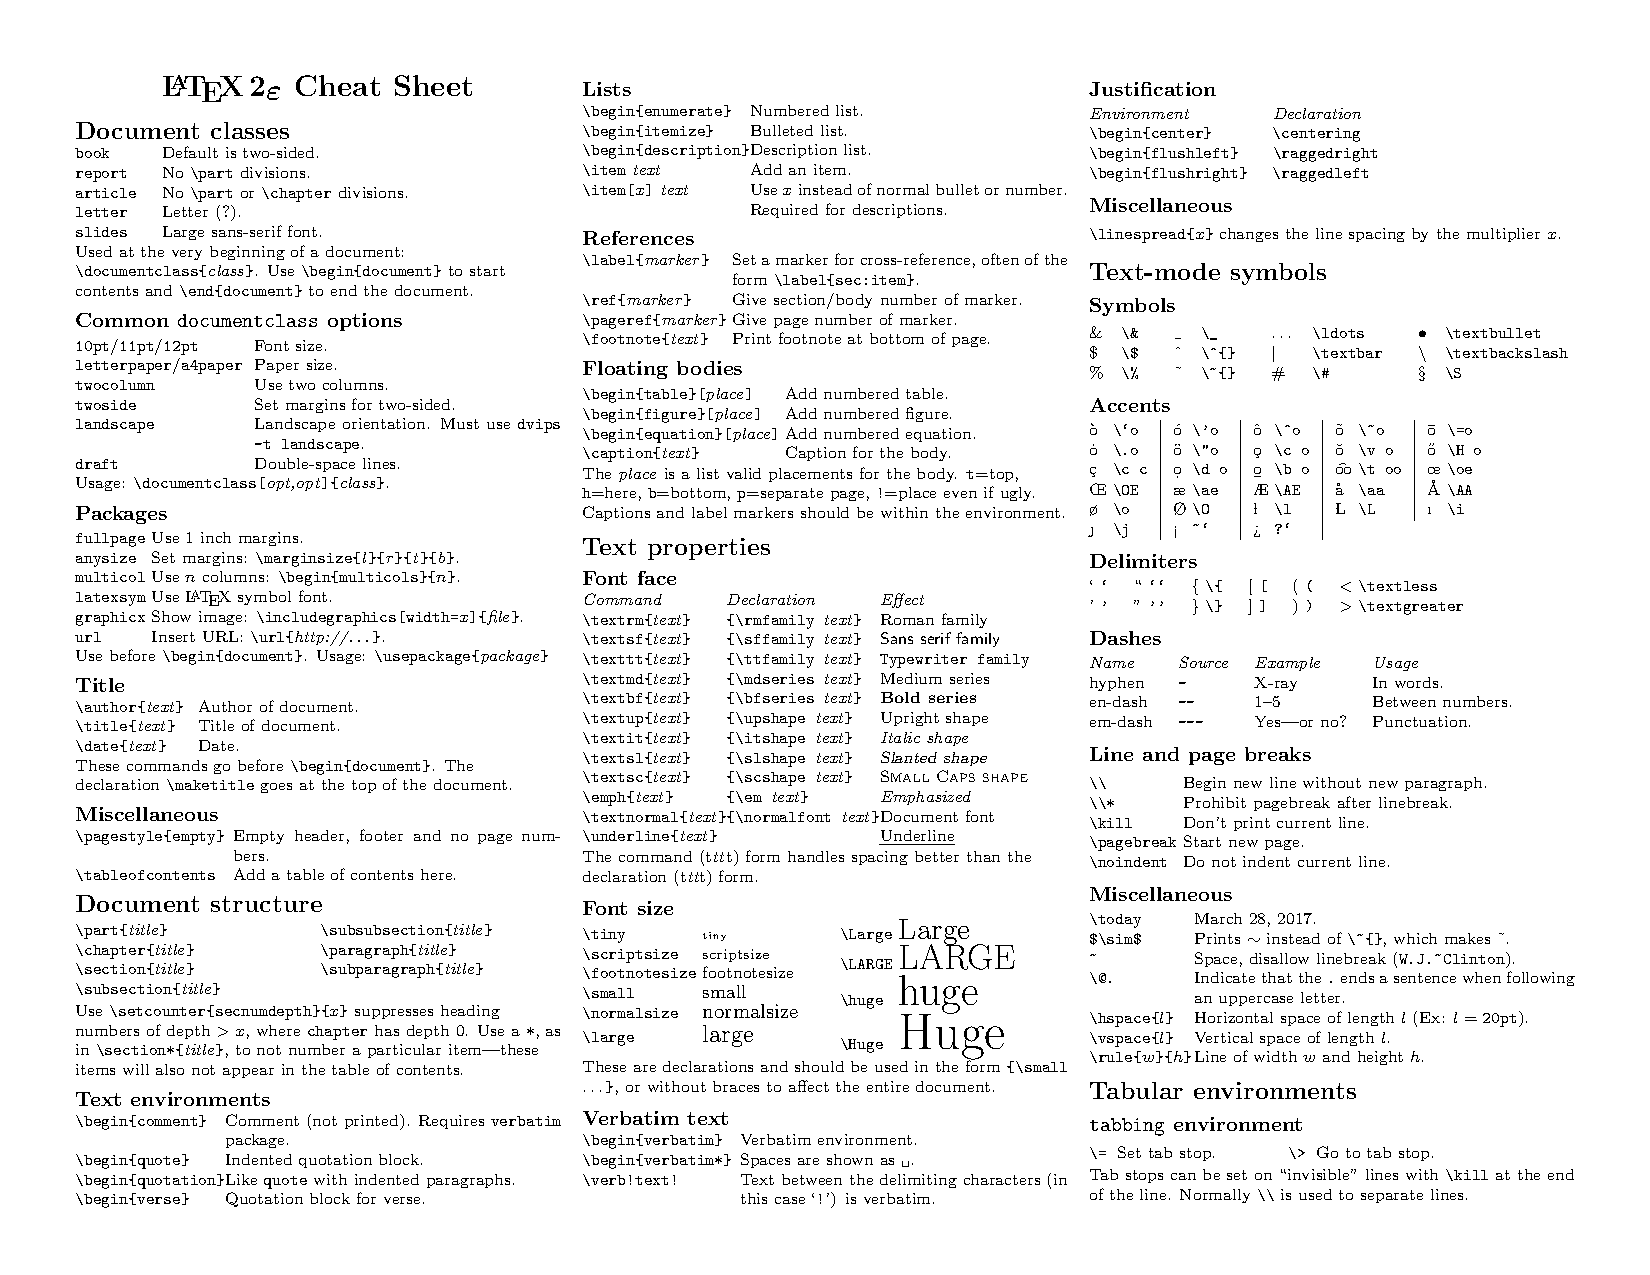
\includepdf[landscape=true,pages=-]{img/latexsheet.pdf} 



\cleardoublepage
